\documentclass[letterpaper,10pt]{article}

\usepackage{enumitem}
\usepackage{titling}
\usepackage{listings}
\usepackage{url}
\usepackage{hyperref}
\usepackage{setspace}
\usepackage{subfig}
\usepackage{sectsty}
\usepackage{pdfpages}
\usepackage{colortbl}
\usepackage{multirow}
\usepackage{multicol}
\usepackage{relsize}
\usepackage{amsmath}
\usepackage{wasysym}
\usepackage{fancyvrb}
\usepackage[yyyymmdd]{datetime}
\usepackage{amsmath,amssymb,amsthm,graphicx,xspace}
\usepackage[titlenotnumbered,noend,noline]{algorithm2e}
\usepackage[compact]{titlesec}
\usepackage{XCharter}
\usepackage[T1]{fontenc}
\usepackage[scaled]{beramono}
\usepackage[normalem]{ulem}
\usepackage{booktabs}
\usepackage{tikz}
\usetikzlibrary{arrows,automata,shapes,trees,matrix,chains,scopes,positioning,calc}
\tikzstyle{block} = [rectangle, draw, fill=blue!20,
text width=2.5em, text centered, rounded corners, minimum height=2em]
\tikzstyle{bw} = [rectangle, draw, fill=blue!20,
text width=4em, text centered, rounded corners, minimum height=2em]

\definecolor{namerow}{cmyk}{.40,.40,.40,.40}
\definecolor{namecol}{cmyk}{.40,.40,.40,.40}
\renewcommand{\dateseparator}{-}

\let\LaTeXtitle\title
\renewcommand{\title}[1]{\LaTeXtitle{\textsf{#1}}}

\lstset{basicstyle=\footnotesize\ttfamily,breaklines=true}

\newcommand{\handout}[5]{
	\noindent
	\begin{center}
		\framebox{
			\vbox{
				\hbox to 5.78in { {\bf ECE 350: Real-Time Operating Systems } \hfill #2 }
				\vspace{4mm}
				\hbox to 5.78in { {\Large \hfill #4  \hfill} }
				\vspace{2mm}
				\hbox to 5.78in { {\em #3 \hfill \today} }
			}
		}
	\end{center}
	\vspace*{4mm}
}

\newcommand{\lecture}[3]{\handout{#1}{#2}{#3}{Lecture#1}}
\newcommand{\tuple}[1]{\ensuremath{\left\langle #1 \right\rangle}\xspace}

\newcommand{\Rplus}{\protect\hspace{-.1em}\protect\raisebox{.35ex}{\smaller{\smaller\textbf{+}}}}
\newcommand{\Cpp}{\mbox{C\Rplus\Rplus}\xspace}


\addtolength{\oddsidemargin}{-1.000in}
\addtolength{\evensidemargin}{-0.500in}
\addtolength{\textwidth}{2.0in}
\addtolength{\topmargin}{-1.000in}
\addtolength{\textheight}{1.75in}
\addtolength{\parskip}{\baselineskip}
\setlength{\parindent}{0in}
\renewcommand{\baselinestretch}{1.5}
\newcommand{\term}{Spring 2023}
\newcommand{\termnumeric}{1235}

\singlespace


\begin{document}

\lecture{ 7 --- Dynamic Memory Allocation }{\term}{Jeff Zarnett}

\section*{Dynamic Memory Allocation}
By now you must surely be familiar with dynamic memory allocation from the perspective of the application developer. To create a new instance of an object in Java, for example, you use the \texttt{new} keyword and the runtime will come and garbage collect it when it is no longer needed. In C++ we have the \texttt{new} and \texttt{delete} operators to allocate and deallocate memory. The \texttt{new} and \texttt{delete} operators invoke the constructor and destructor, respectively. C works on memory at a lower level: to allocate a block of memory in C, there is \texttt{malloc()} and when finished, you return it with \texttt{free()}. This level is a lot closer to the way the operating system thinks about memory: just tell me how much you need and tell me when you are finished with it.

This should square nicely with your experience of using \texttt{malloc()} and \texttt{free()} in C. To allocate an integer, you call \texttt{malloc( sizeof( int ) )}. This creates, somewhere in memory, a new integer and returns its address, which can be stored in a pointer (presumably an integer pointer, but you can store it in a void pointer too). To be sure to ask for the correct amount of memory, we have \texttt{sizeof} which works out the size of its argument (integer) and then the size of an integer, say, 4 bytes, is supplied to \texttt{malloc()}, so 4 bytes are allocated. 

When you \texttt{free()} that pointer, all that happens is that the memory is marked as available, which is why you can sometimes get away with dereferencing a pointer after it has been freed. Sometimes it takes a while for that memory to be reclaimed or reused so the old value just happens to still be there in memory. Note that \texttt{free()} does not specify how much memory is being returned. This means two things: (1) that the operating system is keeping track of each allocated block's size, and (2) that it is not possible to return part of a block.

With the preliminaries about memory allocation out of the way, now it is time to turn our attention to fulfilling the memory allocation requests that we receive. As we will see, this is not a trivial problem. The operating system will try to find some free memory to meet the request. Although running out of memory is a rare thing given the size of main memory in a modern computer, there is still the possibility that some request may not be fulfilled because no block meeting that need is available.

\subsection*{Fixed Block Sizes}
One possibility for how to allocate memory is in fixed block sizes. All blocks of memory allocated are the same size. This does not mean that requests are not of varying size, it just means that all blocks allocated are the same size. If a request comes in for 1 byte, 1 block is allocated. If a request comes in that is, say, 1.5 blocks, 2 blocks are allocated. 

It is immediately obvious when we look at this that some memory is ``wasted''. If 1.5 blocks are requested and 2 blocks are allocated and returned, we are using up an extra 0.5 blocks. This space cannot be used for anything useful (as it shows as allocated). This is a problem called \textit{internal fragmentation} -- unused memory that is internal to a partition. This is obviously going to occur often when fixed block sizes are used, and the bigger each block is, the more memory will be wasted in internal fragmentation. 

\paragraph{One Size of Blocks.} Suppose the system has only one size of blocks, perhaps, 1~KB. To implement this strategy, divide up memory into blocks of this fixed size and maintain a linked list of addresses of all currently available blocks. When a block is allocated, remove its corresponding node from the linked list; when a block is freed, put a node with that address into the linked list. If the list is empty, a memory request cannot be satisfied, and null will be returned. This is definitely fast as we can allocate memory in $\Theta(1)$ time~\cite{mte241}.

\paragraph{Fixed Block Sizes, Multiple Size Options.} Recognizing that some memory allocation requests are bigger than others, it might make sense to have several different block sizes; perhaps 1~KB, 2~KB, and 4~KB. These can generally be allocated and deallocated in $\Theta(1)$ time if we have one linked list for each different size of block~\cite{mte241}.

Unfortunately, fixed block sizes suffer from a lot of internal fragmentation. This may be suitable for embedded systems where simplicity and speed of operations are more important than worrying about wasting memory. It is obvious from working with languages like C that this is not how \texttt{malloc()} works: 1~KB of memory is not allocated to store a 4-byte integer. What we need instead is a variable block size.

\subsection*{Variable Block Sizes}
To a certain extent, variable block sizes are not that different from fixed block sizes; we just take the size of blocks down to the smallest they can be. In a typical system with byte-addressable memory, in a way, the smallest block is one byte. Now we have a different problem: keeping track of what is allocated and what is free.

\paragraph{Bitmaps.} It is possible to divide memory into $M$ units of $n$ bits, and then to create a bit array of size $M$ storing the status of each of those units. If a bit $m$ in $M$ is 0, it means that unit is unallocated; if it is 1 then that unit is allocated. How much memory is lost to this overhead? $100/(n+1)$\% of the memory is used. If a unit is 4 bytes, the bitmap is about 3\% of memory; if it is 16 bytes the bitmap takes about 0.8\% of memory. Finding a block of $k$ bytes requires searching the bitmap for a run of $\frac{8k}{n}$ zeros~\cite{mte241}.

\paragraph{Linked Lists.}
The other approach, as in the case of fixed size blocks, is to use linked lists. The information of the linked list can be stored separately from all memory allocation or as part of the block of memory. Either approach is workable.

After startup, the linked list contains one entry, as all available memory is in one contiguous block. When a memory request is allocated, for example, to allocate 128 bytes, the block is divided up. Suppose we allocate the first 128 bytes. A new entry is placed in the list, at 128 bytes. The node that is added contains the start address, the length of the block, and a bit indicating it is allocated. The unallocated block's node will contain the updated entry: smaller size, new start address, and the bit indicating it is unallocated. When a block is deallocated, we simply find that block in the linked list and set the bit to zero to indicate it is now available again.

A single linked-list approach may be relatively simple to implement, as it does not require moving blocks around too much. However, for a sufficiently-large memory area, this strategy is quite inefficient. With just one list, every memory allocation potentially requires searching the whole list of all blocks. And that becomes slower and slower as there are more allocations, particularly small allocations. Instead, if we only had to search the free list, we could find free memory much faster.

In a typical system there may be a lot of allocation and deallocation of memory. This will probably lead to breaking memory up into smaller pieces. We may end up with a situation where the free blocks are small and spread out, as in the figure below: 

\begin{center}
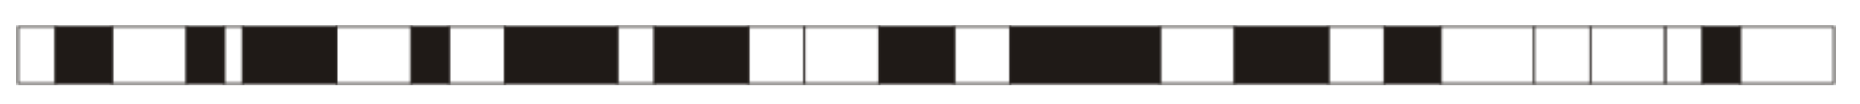
\includegraphics[width=0.9\textwidth]{images/checkerboard.png}\\
Allocated blocks in memory after some time; the ``checkerboard'' situation~\cite{mte241}.
\end{center}

If this happens, it may be that there is a contiguous block of free memory available of size $N$, but this request cannot be fulfilled because the memory is logically split up into smaller pieces. To solve this, we need a way to recombine the split blocks, commonly called \textit{coalescence}. See the updated figure below:

\begin{center}
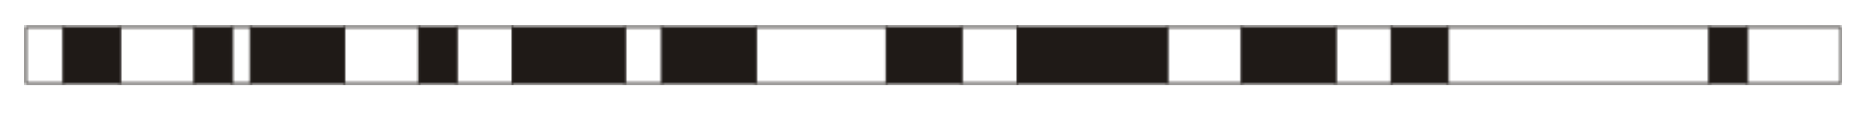
\includegraphics[width=0.9\textwidth]{images/checkerboard-coalesced.png}\\
The ``checkerboard'' situation with the adjacent free blocks coalesced~\cite{mte241}.
\end{center}

\paragraph{Coalescence.} Coalescence is just the process of merging two (or more) adjacent free blocks into one larger block. It also makes sense that dividing memory should be a reversible operation. This solves the problem of a block of $N$ contiguous bytes being unable to be allocated. Coalescence can be done periodically or whenever a block of memory is freed.

As pointed out in~\cite{mte241}, coalescence makes it a good idea to maintain the memory blocks in a doubly-linked list. Recall a linked list has ``next'' pointers connecting the nodes and a doubly-linked list has ``next'' and ``previous'' pointers, to make it easier to traverse the list in both directions. When a block is freed, it may be in the middle of two free blocks, so it is convenient to have previous and next pointers so the adjacent sections can be merged efficiently.

Even with coalescence, we may have the problem that $N$ free bytes exist in the system but spread out over many little pieces, so the request for $N$ cannot be satisfied. When free memory is spread into little tiny fragments, this situation is called \textit{external fragmentation}. It is analogous to internal fragmentation in that there are little bits of space that cannot be used for anything useful, except of course that they are not inside any block (hence external).

\paragraph{External Fragmentation.}
One way to reduce external fragmentation is to increase internal fragmentation. If a request for $N$ bytes comes in and there is a block of $N+k$ available, where $k$ is very small (and unlikely to be allocated on its own), it makes sense to allocate the whole $N+k$ block for the request and just accept that $k$ bytes are lost to internal fragmentation. For example, if a free block contains 128 bytes and the request is for 120 bytes, it may not be worth the hassle and overhead to split this block into 120 and 8, as it is unlikely the 8 bytes will be filled anyway. Some systems round up memory allocations to the nearest power of 2 (e.g., a request for 28 bytes gets moved up to 32). Of course, this does not really help with satisfying the request for $N$ bytes of memory; it just keeps external fragmentation down.

Another idea is \textit{compaction}, which can also be thought of as \textit{relocation}. The goal is simply to move the allocated sections of memory next to one another in main memory, allowing for a large contiguous block of free space. This is a very expensive operation; to do this successfully, the Java runtime, for example, must ``stop the world'' (halt all program execution) while it reorganizes memory. This tends to make Java unsuitable for use in writing a real-time operating system. But even if we are willing to pay the cost, it might not be possible to do.

In previous discussions of memory management from the perspective of the application developer, languages with garbage collection like Java or C\# may do memory compaction as needed when the garbage collector runs. This can work in such languages, because variables are references and unless you are writing an \texttt{unsafe} block in C\#, references can be moved around in memory at the garbage collector or runtime's convenience; all it needs to do is update every reference. This is not the case in languages like C where we operate directly on memory addresses, and thanks to things like pointer arithmetic and using integer variables as addresses, there is no reliable way to update all references. 

The final way we can try to prevent or deal with external fragmentation is through different allocation strategies; that is, how to fit a memory request to a block of free memory. We will examine those strategies now.

\subsubsection*{Variable Allocation Strategies}

Given a memory request of $N$, where do we allocate the memory? If there is no block of at least size $N$, the request cannot be satisfied. If there is only one, the decision is easy. As long as memory has two free blocks of sufficient size ($N$ or more) that cannot be coalesced, a memory allocation request will require making a decision about which of those blocks to split to meet the allocation request. There are five strategies we will examine~\cite{mte241}:

\begin{enumerate}
	\item First fit.
	\item Next fit.
	\item Best fit.
	\item Worst fit.
	\item Quick fit.
\end{enumerate}

As a performance optimization, we could have two linked lists: one for allocated memory and one for unallocated memory. That way to find a free block we do not have to look through the allocated blocks.

\paragraph{First fit.} The strategy of first fit is to start looking at the beginning of memory, and check each block. If the block is of sufficient size, split it to allocate the memory, and return the balance to the unallocated memory list. This algorithm has a runtime of $O(n)$ where $n$ is the number of blocks. This algorithm is simple to implement. 

As referenced earlier, it's important for the sake of efficiency to have separate lists for free and allocated memory. With it, finding a free block is linear in the number of \textbf{free} blocks instead of linear with the number of total blocks -- and most likely the number of allocated blocks is much larger than the number of free blocks. While it may be tempting to have one single linked list because it is easier to implement, that will be dramatically slower.

\paragraph{Next fit.} This strategy is a modification of the first-fit algorithm. Instead of starting at the beginning of memory and finding the first block that meets the request, keep track of where the last block was allocated, and then start the next search after that. This prevents the situation where there are a lot of small unallocated blocks (external fragmentation) all concentrated at the start of memory~\cite{mte241}. The runtime is still $O(n)$, as with first fit.

\paragraph{Best fit.}
Instead of just walking through the list and splitting up the first block equal to or larger than $N$, we could instead try to make a more intelligent decision. Considering all blocks, we choose the smallest block that is at least as big as $N$. This produces the smallest remaining unallocated space at the end. 

This would require either (1) checking every available block ($\Theta(n)$ runtime); or (2) keeping the blocks sorted by increasing size ($O(n)$ runtime). If we use an AVL tree or red-black tree, then we can get best fit to run in $\Theta($ln$(n))$, possibly better runtime than first fit~\cite{mte241}.


\paragraph{Worst fit.}
The problem with best fit is that the leftover bits of memory are likely to be too small to be useful. Rather than trying to find the smallest block that is of size $N$ or greater, choose the largest block of free memory. When the block is split, the remaining free block is, hopefully, large enough to be useful. 

As with best fit, we must either (1) check each available block; or (2) keep the block sorted by size, though decreasing size this time. A max heap is appropriate, or a binomial or Fibonacci heap could also be appropriate~\cite{mte241}.

\paragraph{Quick fit.}
Though not a solution on its own, quick fit is an optimization. If memory requests of a certain size are known to be common, e.g., requests for 1~MB, it might be ideal to keep a separate list of blocks that are of perhaps 1-1.1~MB in size, so that if the request for 1~MB does come in, it can be satisfied immediately and quickly. 



\paragraph{Example: 16~MB Allocation.} The diagram below illustrates where in memory a request of 16~MB may be placed:

\begin{center}
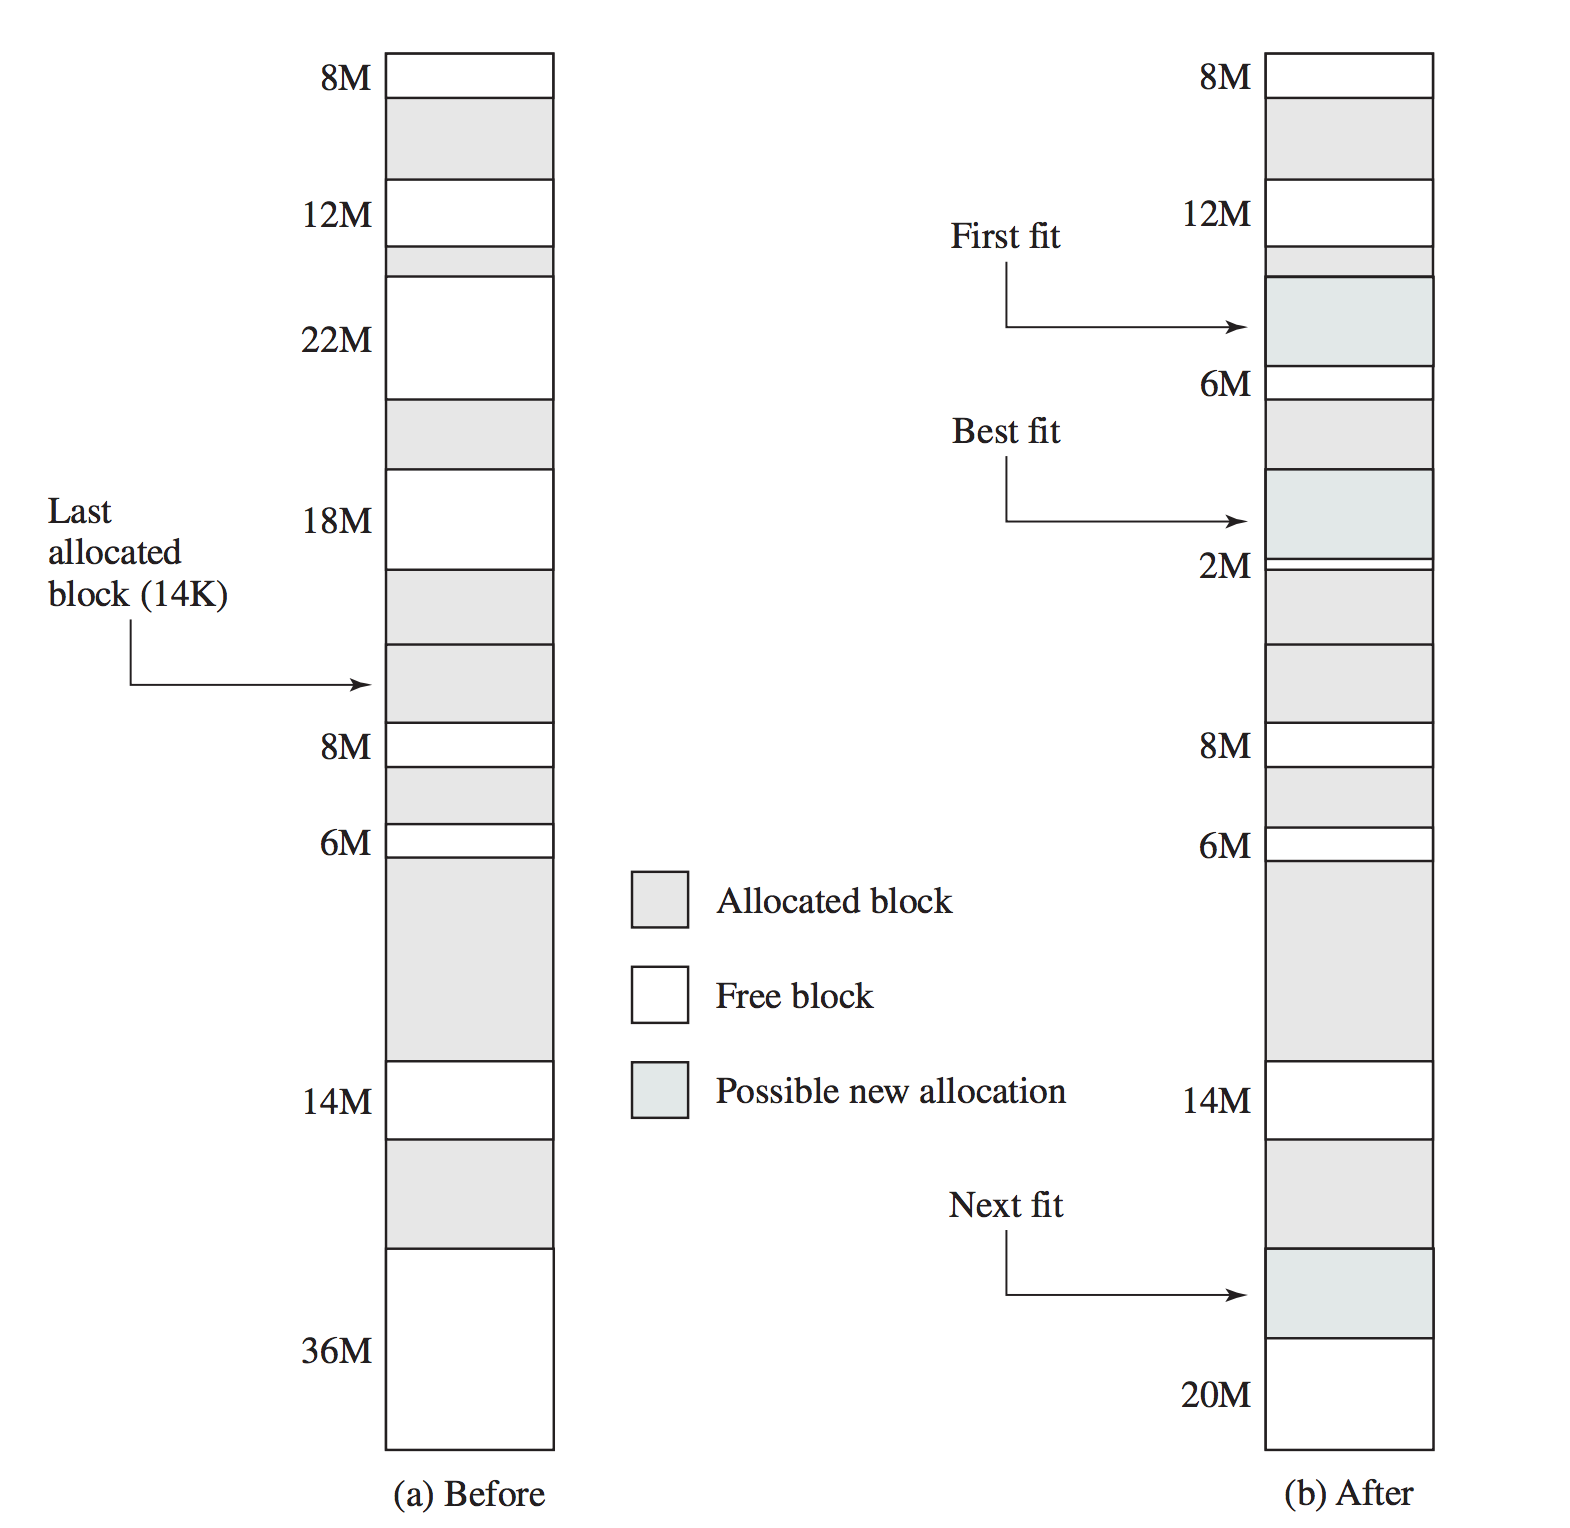
\includegraphics[width=0.50\textwidth]{images/first-best-next.png}\\
An example of where the first, best, and next fit algorithms would place an allocation~\cite{osi}.
\end{center}

The worst fit algorithm is not shown, but it would overlap with the placement indicated for next fit, because the largest block of free space before the allocation is is 36M.

\subsubsection*{Choosing a Strategy}

According to~\cite{osc}, simulations show that worst fit performs, well, worst in terms of time required to fulfill an allocation request and that it results in the most wasted space. The performance problems of worst fit can be fixed, of course, by keeping the memory blocks in a max heap, but that still does not address the wasted space problem. First (next) and best fit are about equal in how well they utilize memory, but first fit tends to be faster. Despite this, even with optimization, given $x$ allocated blocks, another 0.5$x$ blocks may be lost to fragmentation.

This is supported by~\cite{osi}, whose analysis also indicates that first fit is the fastest and best algorithm. The next fit algorithm tends to do allocations at the end of memory, so the largest block of free memory (typically at the end) is quickly broken up. On the other hand, first fit tends to litter the beginning of memory with small fragments. Best fit tends to produce free blocks that are too small to be useful. 

\subsubsection*{Advanced Strategy: Binary Buddy}
Now let us examine a compromise between fixed and variable allocation, as laid out in~\cite{osi}. There is some internal fragmentation, but it is a trade-off against how much external fragmentation we are willing to accept.

In a buddy system, memory blocks are available in powers of 2. More formally, a block is of size $2^{K}$, where $L \leq K \leq U$ and $2^{L}$ is the smallest block size that can be allocated and $2^{U}$ is the largest block size that can be allocated (usually the full size of memory). 

Initially, memory is treated as a single block of size $2^{U}$. If a request of size $n$ occurs such that $2^{U-1} < n \leq 2^{U}$, then the entire block is allocated. Otherwise, the block is split into two ``buddies'', of size $2^{U-1}$. If $2^{U-2} < n \leq 2^{U-1}$, allocate one of the blocks of $2^{U-1}$ to the request. Otherwise, subdivide again. Repeat until the smallest block greater than or equal to $n$ is allocated. 

In subsequent allocations, we look through the data structure, typically a tree, to find either (1) a block of appropriate size; or (2) a block that can be subdivided to meet the allocation. Whenever a pair of buddies (two blocks of equal size, split from the same ``parent'') in the list are both free, they can be coalesced.

Consider the example below where a 1~MB block is allocated using the Binary Buddy system.

\begin{center}
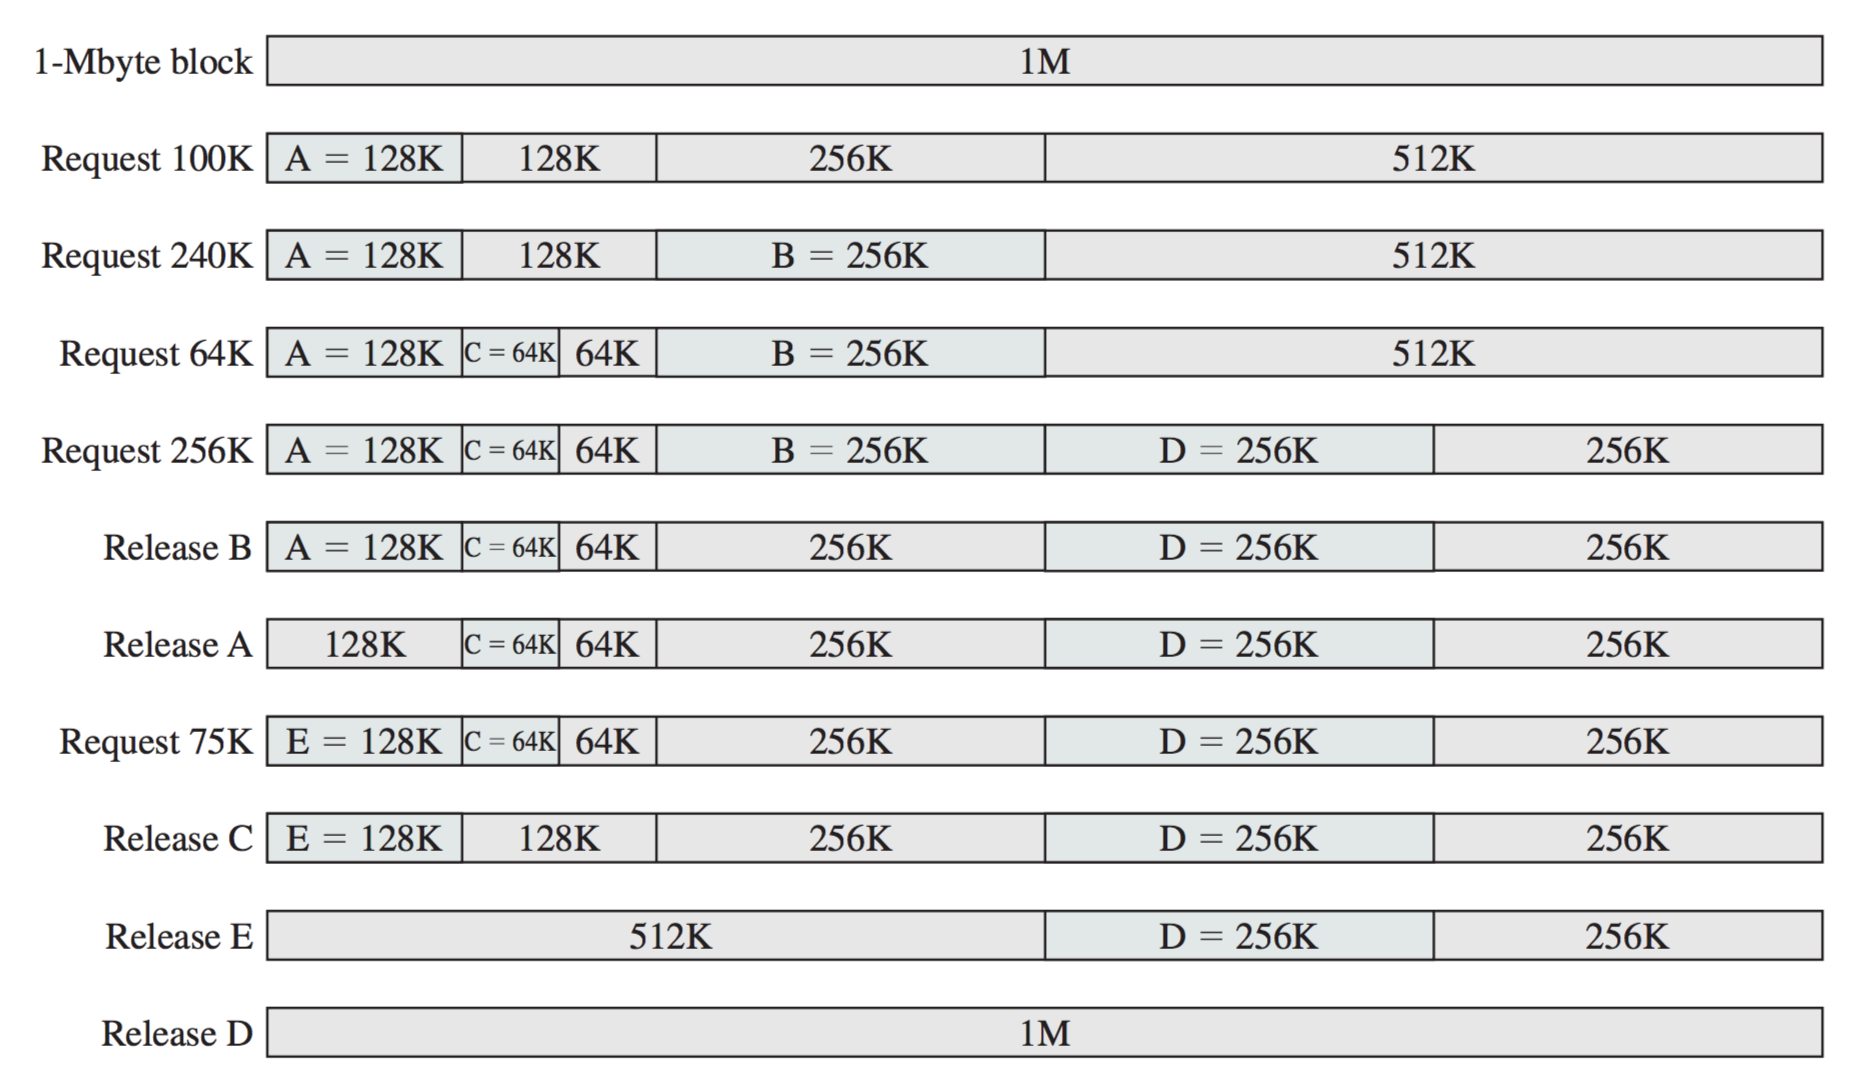
\includegraphics[width=0.80\textwidth]{images/binary-buddy.png}\\
An example of the Binary Buddy system for memory allocation~\cite{osi}.
\end{center}

\bibliographystyle{alphaurl}
\bibliography{350}


\end{document}
